\documentclass{article}
\usepackage[utf8]{inputenc}
\usepackage[spanish]{babel}
\usepackage{hyperref}
\usepackage{natbib}
\usepackage{amsmath}
\usepackage{caption}
\usepackage{subcaption}
\bibliographystyle{abbrv}
\usepackage{graphicx}
\graphicspath{ {Images/} }

\title{Desarrollo de una Red Neuronal Convolucional para la detección y clasificación de ondas P300\\
Trabajo Práctico \\
Redes Neuronales Profundas}
\author{Juan Carlos Suárez Barón \\
Juan Manuel Pérez}
\date{Deciembre 2017}



\begin{document}

\maketitle

\section{Introduccion}

En este trabajo, se implementó un clasificador basado en una Red Convolucional Profunda para la de detección de un potencial evocado por un estímulo (Event-Related Potential, ERP). Para ello, se utilizó un dataset obtenido durante un experimento llevado a acabo en una exposición con un headset de bajo costo, lo cual permite experimentar esta técnica en un ambiente no tan controlado y más ruidoso.

\subsection{P300}

Los potenciales relacionados con eventos (Event-related potential, o ERP) son la medida de las respuestas cerebrales a eventos cognitivos, sensoriales o motores específicos. Uno de los principales enfoques relacionados con las interfases cerebro-computadora (BCI) se basa en los ERP.

Un tipo de onda bien estudiada es el P300. El potencial evocado P300 corresponde a la presencia de un pico de voltaje, del orden los uV, con una latencia cercana a los 300 ms, como se puede apreciar en la figura \ref{fig:P300Wave}. Este potencial se presente ante un estímulo visual, auditivo o sensorial ``infrecuente'', es decir, que ocurre con menor probabilidad que otros estímulos más frecuentes, a los cuáles llamaremos distractores \cite{Amiri2013ARO}.

\begin{figure}[t]
    \centering
    \begin{subfigure}{.45\textwidth}
        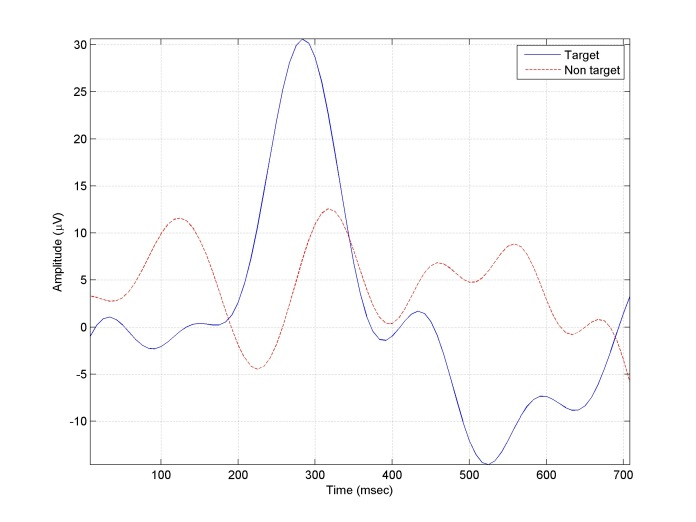
\includegraphics[width=\textwidth]{P300Wave.jpg}
        \subcaption{ Patrón temporal del componente P300..}
        \label{fig:P300Wave}
    \end{subfigure}
    
    \begin{subfigure}{.45\textwidth}
        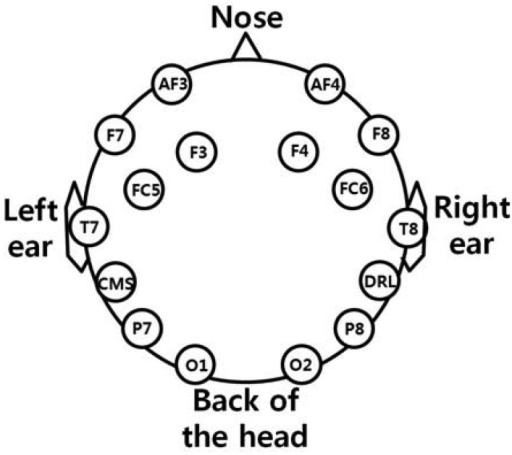
\includegraphics[width=\textwidth]{emotiv}
        \subcaption{ Loocalización de los electrodos usados para la detección de los P300.}
        \label{fig:ElectrodeMap}
    \end{subfigure}
    
\end{figure}


\subsection{P300 Speller}

 
\begin{figure}[t]
    \centering
    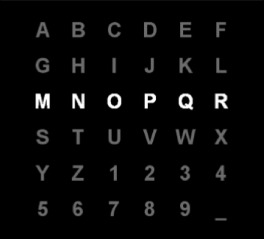
\includegraphics{Matrix6x6.jpg}
    \caption{Configuración típica de un P300 BCI con relimentación visual.}
    \label{fig:Matrix6x6}
\end{figure}

El potencial evocado P300 ha demostrado ser una señal confiable para controlar un BCI. En \cite{farwell1988talking} se describe el P300 Speller, un método de deletreo mediante BCI. Consiste en una matriz de caracteres de $6 \times 6$ como se muestra en la figura \ref{fig:Matrix6x6}. Esta matriz se presenta en la pantalla de la computadora. El usuario centra su atención en un carácter para seleccionarlo, mientras de manera aleatoria se van iluminando las 6 filas y 6 columnas. La fila o columna parpadeante correspondiente al caracter seleccionado evoca la respuesta P300. Las filas y columnas distractoras no contribuyen a generar P300. Como observamos, la frecuencia de aparición de este potencial evocado es de 1/6, ya que sólo una de las filas y una de las columnas es la objetivo mientras las demás son distractoras.

Mediante un algoritmo de clasificación, podemos predecir la probabilidad de ocurrencia de este potencial en el intervalo medido. En base a repetidos intentos (iluminando varias veces cada fila y cada columna) se puede obtener con relativa precisión el caracter en cuestión
\section{Materiales y Métodos}

Como parte de la metodología para llevar a a cabo el experimento se tomó como base el esquema de la figura 1, en el que se destacan tres fases del proceso de detección de patrones a partir del electroencefalograma o EEG: Pre-procesamiento de la señal, extracción y clasificación de características. El primer paso cosnsiste en  eliminar el ruido, como los artefactos o el ruido de la línea de alimentación que se agrega al EEG.

En nuestro caso, no llegaremos a la predicción del caracter, sino tan sólo nos quedaremos con la clasificación de los P300.

\begin{figure}[t]
    \centering
    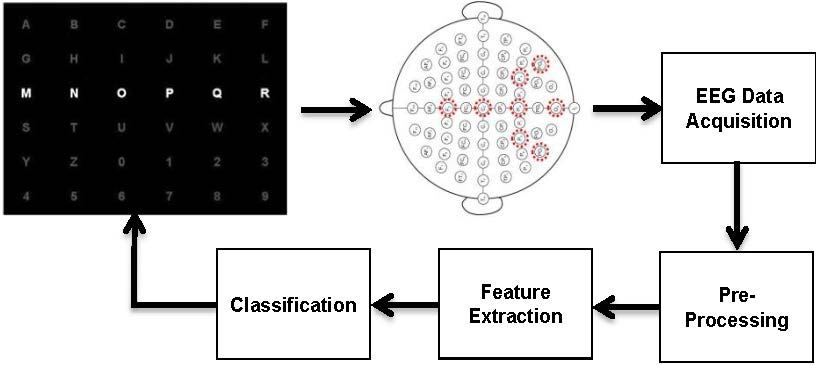
\includegraphics[width=\textwidth]{P300BCI.jpg}
    \caption{Configuración típica de un P300 BCI con relimentación visual.}
    \label{fig:P300BCI}
\end{figure}


\subsection{Dataset}

El dataset consiste en grabaciones hechas en \emph{Tecnópolis}. 135 sujetos participaron del experimento, que consistió en deletrear palabras preestablecidas para calibrar el sistema (etapa de entrenamiento), y luego un modo \emph{free-riding} en el cual los sujetos podían utilizar el speller libremente. Sólo se recopiló la parte de entrenamiento.

En cada paso, una de las filas o columnas de la matriz del speller \ref{fig:Matrix6x6} se intensifica aleatoriamente durante 100 ms. A continuación, todas las filas y columnas se desactivaron durante 75 ms. Esto continúa hasta que se enciendan 12 filas y columnas para cada carácter. 

Se utilizó un EMOTIV, un headset de bajo costo que consiste sólo de 14 electrodos, con un sampling rate de 128 hz. Se aplicó un filtro FIR de fase cero entre 0 y 20 hz. 

La señal de EEG se separó en instancias (epochs) de la siguiente manera: por cada estímulo (flash en la matriz de letras) se tuvo en cuenta los 100 ms previos (utilizados para la estabilización de la señal) y los 700 restantes al estímulo. Es decir, si el estímulo ocurrió en tiempo $t$, se obtuvo la instancia $(t-100, t+700)$. Esto nos da 104 muestras por los 14 canales.

Para el tratamiento de los archivos resultantes, se utilizó la librería de Python \emph{MNE} \cite{gramfort2014mne}.


\subsection{Normalización}

Para mejorar la performance del clasificador, trasladamos y re-escalamos los datos de la siguiente manera:

\begin{equation*}
    I_{i, j} = (I_{i, j} - \bar{I_i}) / \sigma_i
\end{equation*}
    
donde $I(i, j)$ representa el voltaje medido en el electrón $i$ en tiempo $j$, $ \bar{I_i})$ y $\sigma_i$ representan el valor medio y la desviación estándar del electrón $i$. Estas normalizaciones se efectuaron por sujeto. 


\subsection{Topología de la Red}

La red consta de dos capas convolucionales, seguidas de una capa densa y finalmente de una salida que indica la probabilidad de que la entrada se corresponda con un potencial P300. 

De manera similar a lo que suele hacerse en el área de BCI, nuestra red efectúa: en primer lugar se buscan combinaciones óptimas de canales, para luego efectuar una extracción de características en base a patrones (por ejemplo, Fourier y Wavelets). En ese sentido, la estructura de la red es bastante comprensible.

Las capas convolucionales que implementan dichos filtrados (primero en espacio y luego en tiempo) son o bien vectores columna o fila, para evitar que el filtrado se centre en electrodos que no tienen continuidad espacial. 

Así, la topología de la red es la siguiente:

\begin{itemize}
    \item $L_0$: Capa de entrada, $I_{i,j}$ con tamaño $14 \times 104$.
    \item $L_1$: Capa convolucional, con 12 filtros de tamaño $(14, 1)$. \item $L_2$: Capa convolucional, con 60 filtros de tamaño $(1, 13)$.
    \item $L_3$: Capa densa, totalmente conexa a la capa anterior.
    \item $L_4$: Capa de salida, consta de una neurona.
\end{itemize}

Las funciones de activación utilizadas son \emph{reLU} para todas las capas, salvo para la salida que utiliza una función de activación sigmoidea.

Esta topología (a la que denominaremos $CNN-1$) fue la básica. Probamos otras combinaciones:

\begin{itemize}
    \item $CNN-2$: Agregamos una capa de \emph{max-pooling} inmediatamente después de la segunda capa convolucional.
    \item $CNN-3$: Dos capas convolucionales seguidas de \emph{max-pooling}
\end{itemize}

\subsubsection{Entrenamiento y regularización}

La red se entrenó utilizando el algoritmo \emph{rmsprop}\cite{tieleman2012lecture} con \emph{entropía cruzada} como función de pérdida. Para evitar el overfitting, utilizamos en conjunto dos técnicas:

\begin{itemize}
    \item Early Stopping: Se separó un pequeño subconjunto de validación para ir verificando que por cada \emph{epoch} (en el sentido de Redes Neuronales) la función de pérdida tenga una mejora. Si no es así luego de 3 epochs, se detiene el entrenamiento
    \item Dropout: con cierta probabilidad $p$, se ponen, en un paso del entrenamiento, a 0 las entradas de una capa. Esto evita que las unidades se ``co-adapten'' demasiado.
\end{itemize}

Se utilizó la librería de Python \emph{keras}\cite{chollet2015} para su implementación.

\section{Resultados}

En la tabla \ref{tab:scores} podemos observar los resultados obtenidos por el clasificador. Se midieron la efectividad (accuracy), precisión, exactitud (recall) y área bajo la curva ROC. 

\begin{table}[t]
    \centering
    \begin{tabular}{|c|c|c|c|c|}
        \hline
        Clasificador & Accuracy & Precision & Recall & ROC AUC  \\\hline
        CNN-1 & 0.55 & 0.21 & 0.65 & 0.64 \\
        CNN-2 & 0.59 & 0.23 & 0.61 & 0.64 \\
        CNN-3 & 0.52 & 0.22 & 0.72 & 0.66 \\
        \hline 
    \end{tabular}
    \caption{Resultados de la clasificación}
    \label{tab:scores}
\end{table}

A su vez, por la topología planteada, es posible analizar los filtros obtenidos en la primer capa. Estos representan combinaciones de electrodos que resultaron del entrenamiento de la red. En la figura \ref{fig:kernels} se pueden apreciar los pesos obtenidos para algunos de los filtros entrenados


\begin{figure}
    \centering
    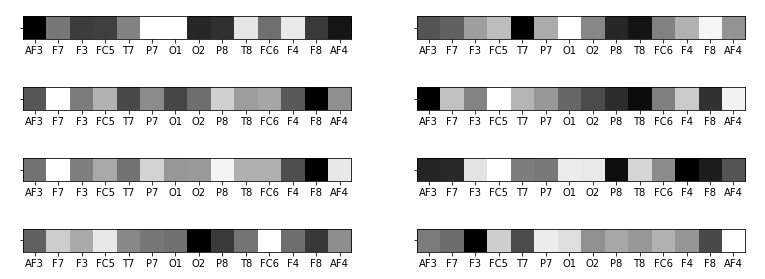
\includegraphics[scale=0.5]{channel_filters.png}
    \caption{Filtros espaciales obtenidos. Más oscuro implica más peso}
    \label{fig:kernels}
\end{figure}


\section{Discusión y trabajo a futuro}

Los resultados obtenidos en este trabajo se asemejan a los de \cite{cecotti2011}; sin embargo, es de notar que nuestros datos son de calidad sensiblemente menor ya que fueron tomados por equipamiento con mucha menor resolución espacial y temporal. A su vez, las condiciones de recolección de los datos son mucho más ruidosas.

Sin embargo, los resultados son interesantes ya que pueden permitirnos pre-entrenar una red neuronal profunda para detectar P300 con alta precisión, ajustando las capas finales de acuerdo a cada usuario.

Como trabajo a futuro, nos queda analizar un poco mejor los datos para sacar aquellos muy ruidosos, refinar datos haciendo una selección de los mejores electrodos. A su vez, queda efectuar la detección del caracter, que es la tarea usualmente medida en esta aplicación de BCI.




\bibliography{Referencias}
\end{document}
